\subsection{Red de grafos generada por el RNA}

	La información exportada en el Código \ref{lst:EJ5_5}, Código \ref{lst:EJ5_6} y Código \ref{lst:EJ5_7} es utilizada resumida por el RNA para una mejor interpretación. El resultado de este resumen se ilustra en el diagrama de la Figura \ref{fig:EJ5_8}.
	
	\begin{figure}[H]
		\centering
		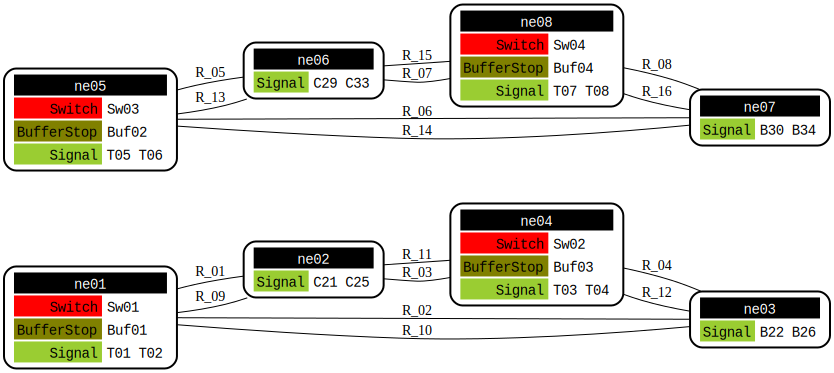
\includegraphics[width=1\textwidth]{Figuras/Graph_5}
		\centering\caption{Red de grafos generada por el RNA para el ejemplo 5.}
		\label{fig:EJ5_8}
	\end{figure}
	
	Cada nodo del grafo de la Figura \ref{fig:EJ5_8} corresponde a un \textit{netElement}. En cada nodo se listan todos los elementos ferroviarios contenidos por en \textit{netElement}. Las aristas del grafo son las rutas que los conectan. De esta manera, es posible detectar visualmente que los grafos que definen ambas vías principales son disconexos, compatibles con lo esperado en base a la Figura \ref{fig:EJ5_1}.